\documentclass{cernatlasnote}
\usepackage[T1]{fontenc}
\usepackage[utf8]{inputenc}
\usepackage{lmodern}
\usepackage{graphicx}
\usepackage{booktabs}
\usepackage{array}
\usepackage{longtable}
\usepackage{enumitem}
\usepackage{tikz}
\usetikzlibrary{arrows.meta,positioning,fit,calc}
\hypersetup{hidelinks,pdftitle={DUNE SC-PDS-DPS ICD: Physical Layer and Protocols},pdfauthor={Manuel Arroyave}}
\setlength{\emergencystretch}{3em}
\setlength{\parindent}{0pt}
\setlength{\parskip}{0.4em}
\setlength{\tabcolsep}{4pt}
\renewcommand{\arraystretch}{1.13}
\setlist[itemize]{leftmargin=1.3em,itemsep=0.15em,topsep=0.25em}
\newcolumntype{L}[1]{>{\raggedright\arraybackslash}p{#1}}
\newcommand{\code}[1]{\nolinkurl{#1}}
\newcommand{\pending}{\textit{To be specified}}
\definecolor{duneblue}{HTML}{1B4E8A}
\definecolor{dunegreen}{HTML}{35704C}
\tikzset{box/.style={draw=duneblue,rounded corners=2pt,fill=duneblue!5,align=center,font=\small,inner sep=7pt},flow/.style={-{Latex[length=2mm]},thick},both/.style={{Latex[length=2mm]}-{Latex[length=2mm]},thick}}

\title{DUNE Interface Control Document:\\Slow Controls, Photon Detector System\\and Detector Protection System}
\author{}
\date{17 September 2026}
\EDMSDocNo{SC--PDS--DPS ICD}
\EDMSDocId{To be assigned}
\draftversion{0.1 --- physical layer and protocols}
\documentlabel{17 September 2026}
\DocAuthors{Manuel Arroyave}
\DocCheckedBy{Pending review}
\DocApprovedBy{Pending approval}

\begin{document}
\maketitle
\begin{abstract}
This draft defines the physical connection and protocol architecture of the
PDS interface to Slow Controls, DAQ and DPS. Each DAPHNE has one 1\,Gb Ethernet
connection for control, configuration and monitoring, through a network switch
to physical server infrastructure. DAQ configuration is integrated into the
external OPC UA server; Hermes remains a separate protocol service on the same
DAPHNE Ethernet connection. The FD-VD baseline is 1,344 PDS channels, with
32 allocated channels per board and 42 DAPHNE boards.

The document identifies protocol endpoints, the initiator of each exchange,
request/reply and publication behavior, shared resources and the specifications
needed for implementation. This first draft is limited to the physical layer
and protocols. It is submitted for interface review.
\end{abstract}
\vfill
\makereviewtable
\clearpage
\tableofcontents
\clearpage
\section{Physical layer}
\label{sec:physical}

\subsection{Connection inherited from the DAQ--PDS ICD}

The physical CCM interface is taken from the \emph{Control, Configuration, and
Monitoring (CCM)} subsection of the DAQ--PDS ICD, EDMS 2088726, as maintained in
\code{daphne-icd} [R1, R2]:

\begin{quote}
Each DAPHNE and each LCM provides a dedicated 1\,GbE SFP link reserved for CCM
(no data readout on this link).

Fibers up to the PDS mini-rack patch panels are provided by PDS; continuation
and active switching are coordinated with DAQ and Technical Coordination.
\end{quote}

For DAPHNE, this means \textbf{one board Ethernet connection} shared by its
control, configuration and monitoring services. The physical path is:
\begin{center}
\textbf{DAPHNE Ethernet interface $\longleftrightarrow$ switch
$\longleftrightarrow$ physical server.}
\end{center}
The switch forwards Ethernet traffic to the appropriate server interface.
OPC UA, ZeroMQ, Protobuf and IPBus describe software communication carried by
the network. The OPC UA server is software deployed on physical server
infrastructure; it is not the name of a board connector or a separate cable.

\subsection{FD-VD inventory}

\begin{longtable}{L{0.48\textwidth}L{0.45\textwidth}}
\caption{FD-VD channel and board inventory.}\\
\toprule
\textbf{Item} & \textbf{FD-VD baseline} \\
\midrule
\endhead
PDS channels & 1,344 \\
Channels allocated to each DAPHNE & 32 \\
DAPHNE boards & $1,344/32=42$ \\
DAPHNE CCM connections & 42 board connections, one per board \\
Membrane PDS & 352 tiles, two channels per tile: 704 channels [R2] \\
Cathode PDS & 320 tiles, two channels per tile: 640 channels [R2] \\
\bottomrule
\end{longtable}

The membrane and cathode populations add to 1,344 channels. Membrane devices
use conductive power and electrical signal paths; cathode devices use
Power-over-Fiber and optical signal transmission [R2]. Both reach the same
DAPHNE CCM boundary. The installed mapping shall identify the population
served by each board. The 32-channel allocation is the FD-VD system mapping.

Servers, switches, PoF, LCM and power-supply units have separate installation
inventories.

\subsection{Physical topology and server boundary}

\begin{figure}[htbp]
\centering
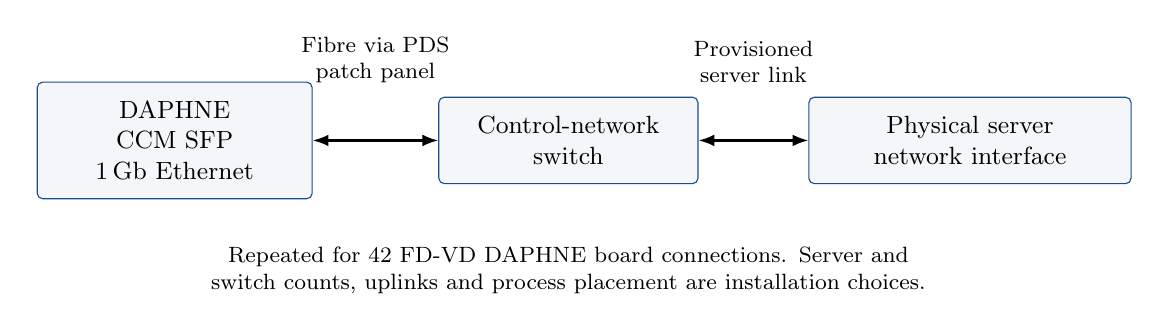
\begin{tikzpicture}
\node[box,text width=30mm] (board) at (0,0)
 {DAPHNE\\CCM SFP\\1\,Gb Ethernet};
\node[box,text width=28mm] (switch) at (5.0,0)
 {Control-network\\switch};
\node[box,text width=36mm] (host) at (10.1,0)
 {Physical server\\network interface};
\draw[both] (board) -- node[above,yshift=6mm,align=center,font=\footnotesize]
 {Fibre via PDS\\patch panel} (switch);
\draw[both] (switch) -- node[above,yshift=6mm,align=center,font=\footnotesize]
 {Provisioned\\server link} (host);
\node[font=\footnotesize,align=center,text width=135mm] at (5.0,-1.65)
 {Repeated for 42 FD-VD DAPHNE board connections. Server and switch counts,
 uplinks and process placement are installation choices.};
\end{tikzpicture}
\caption{Physical CCM connection. Software-service placement is shown separately
in Figure~\ref{fig:protocol}.}
\end{figure}

The external OPC UA server hosts the integrated DAQ configuration component
and the Protobuf/ZeroMQ client of the DAPHNE service. Ignition connects as an
OPC UA client. The Hermes client remains separate from this OPC UA server.
It may run on the same physical host or another DAQ host; in either case its
traffic reaches the same board Ethernet interface. Software separation does
not require a second DAPHNE network connection.

SC provides computing infrastructure for its DCS processes.
PDS, SC and DAQ shall record the physical hosts for the
integrated OPC UA/configuration server and the separate Hermes client, with
installation and support assignments. The DPS controller and its physical I/O
require their own endpoint description.

\subsection{Physical interface specification}

\begingroup\small
\begin{longtable}{L{0.23\textwidth}L{0.38\textwidth}L{0.31\textwidth}}
\caption{CCM physical specification and remaining installation details.}\\
\toprule
\textbf{Element} & \textbf{Defined baseline} & \textbf{Installation detail to record} \\
\midrule
\endhead
DAPHNE port & One 1\,GbE SFP CCM link per board, copied from DAQ--PDS. & Board port label and installed SFP part number. \\
PDS fibre and patching & PDS supplies fibres to its mini-rack patch panels. & Fibre type, connector, wavelength, length, patch route and link budget. \\
Switch board-facing port & Compatible Ethernet termination for the board's 1\,GbE link. & Switch/port identity, compatible optic, agreed duplex and negotiation settings. \\
Switch uplinks & Carry the aggregate CCM traffic to the server network. & Topology, line rates, contention points and redundancy arrangement. \\
Physical server interface & Ethernet NIC connected to the provisioned control network. & Host/NIC identity, port, medium, rate and assignment to the server process. \\
\bottomrule
\end{longtable}
\endgroup

The cited CCM paragraph specifies an SFP link but does not supply the complete
CCM optical specification. The timing and 10\,GbE readout optical specifications
in DAQ--PDS apply to their respective links and shall not be copied into the
CCM link specification. Final installation drawings shall resolve the open
physical details above using the selected equipment.

The 1\,Gb/s line rate is shared by all enabled services on each board connection.
Uplink and server capacity shall be sized from the combined traffic and
concurrent operations in Section~\ref{sec:contention}.

DAQ acquisition data and the optical DTS signal retain the separate physical
interfaces defined by DAQ--PDS [R1, R2]. Here they are referenced only to identify
what their configuration and software services do over the shared CCM link.

Installation checks shall identify all 42 board routes and establish media
compatibility, link operation and simultaneous DAPHNE/Hermes reachability
from the actual external server infrastructure.

\section{Control, configuration and monitoring protocols}

\subsection{Service architecture}

SC provides the OPC UA server and control arbitration. The server hosts DAQ
configuration and forwards publications from
\code{daphne-server}: equipment monitoring to Ignition; firmware counters,
timing state and applied readout configuration to DAQ opmon.
Hermes receives configuration over UDP/IPBus. Figure~\ref{fig:protocol} shows
the DAPHNE path; box interfaces are defined in Section~\ref{sec:boxes}.

\begin{figure}[htbp]
\centering
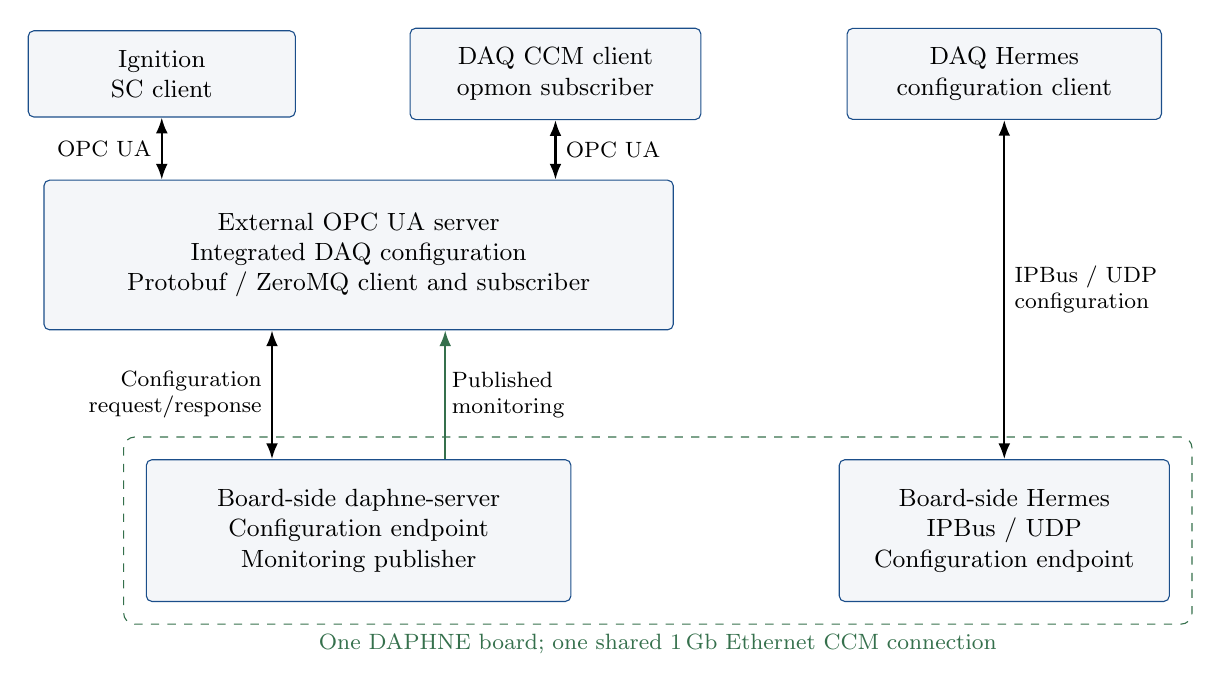
\begin{tikzpicture}
\node[box,text width=29mm] (ignition) at (0,0) {Ignition\\SC client};
\node[box,text width=32mm] (daq) at (5.0,0) {DAQ CCM client\\opmon subscriber};
\node[box,text width=35mm] (hermesclient) at (10.7,0)
 {DAQ Hermes\\configuration client};
\node[box,text width=75mm,minimum height=19mm] (ua) at (2.5,-2.3)
 {External OPC UA server\\Integrated DAQ configuration\\Protobuf / ZeroMQ client and subscriber};
\node[box,text width=49mm,minimum height=18mm] (daphne) at (2.5,-5.8)
 {Board-side daphne-server\\Configuration endpoint\\Monitoring publisher};
\node[box,text width=37mm,minimum height=18mm] (hermes) at (10.7,-5.8)
 {Board-side Hermes\\IPBus / UDP\\Configuration endpoint};
\node[draw=dunegreen,dashed,rounded corners,fit=(daphne)(hermes),inner sep=8pt,
 label={[font=\footnotesize,text=dunegreen]below:One DAPHNE board; one shared 1\,Gb Ethernet CCM connection}] {};
\draw[both] (ignition) -- node[left,font=\footnotesize]{OPC UA} (ignition |- ua.north);
\draw[both] (daq) -- node[right,font=\footnotesize]{OPC UA} (daq |- ua.north);
\draw[both] ([xshift=-11mm]ua.south) -- node[left,align=right,font=\footnotesize]
 {Configuration\\request/response} ([xshift=-11mm]daphne.north);
\draw[flow,draw=dunegreen] ([xshift=11mm]daphne.north) -- node[right,align=left,font=\footnotesize,fill=white,inner sep=2pt]
 {Published\\monitoring} ([xshift=11mm]ua.south);
\draw[both] (hermesclient.south) -- node[right,align=left,font=\footnotesize]
 {IPBus / UDP\\configuration} (hermes.north);
\end{tikzpicture}
\caption{DAPHNE CCM configuration and published monitoring.}
\label{fig:protocol}
\end{figure}

\subsection{Configuration exchanges}

DAQ CCM requests run-variable and timing-endpoint configuration through OPC UA.
The server exchanges Protobuf
messages over ZeroMQ and TCP using a DEALER client and the board's ROUTER
endpoint [R3, R4].
The reference port is TCP 40001 [R5]. Correlated responses shall distinguish
acceptance, completion and failure.

Hermes retains its independent IPBus/UDP configuration endpoint, reference
UDP 50001 [R6], outside the OPC UA server. Both services share the board
connection and gateware lifecycle.

\subsection{Published monitoring}

Monitoring shall be published periodically or on change, without a client
request for each update. Only configuration and control operations, including
reset/recovery commands, use application request/response. Local hardware
sampling is performed by the producing service.

The proposed DAPHNE publication transport is Protobuf over ZeroMQ PUB/SUB over TCP,
using endpoints separate from configuration. The OPC UA server subscribes to
\code{daphne-server} publications and distributes them through OPC UA
subscriptions. Opmon monitoring follows the path
\code{daphne-server} $\rightarrow$ OPC UA server $\rightarrow$ DAQ opmon.

\begin{center}\small
\begin{tabular}{L{0.25\textwidth}L{0.68\textwidth}}
\toprule
\textbf{Consumer} & \textbf{Monitoring responsibility} \\
\midrule
DAQ opmon & Firmware counters, timing state and applied data-readout configuration, published by \code{daphne-server} through OPC UA. \\
SC / Ignition & Voltages, temperatures, fans, service status and software/firmware versions. \\
SC and DAQ & Timing-endpoint condition, reset/recovery progress and board readiness. \\
\bottomrule
\end{tabular}
\end{center}

Opmon shall not acquire voltage monitoring. SC receives equipment monitoring
through the OPC UA server without an opmon dependency. Publications shall
carry source identity, time, sequence and validity. Subscribers shall detect
stale or missing updates and obtain a current snapshot after reconnecting.

\subsection{Timing-endpoint control and recovery over GbE}

Timing-endpoint configuration follows the DAQ configuration path:
\begin{center}
DAQ $\longleftrightarrow$ OPC UA server $\longleftrightarrow$
DAPHNE service $\longleftrightarrow$ local timing endpoint.
\end{center}
The same interface shall expose reset and recovery to authorized SC clients.
Timing monitoring shall be published over the board's GbE connection and
made available to both SC and DAQ.

A reset request shall identify its target and receive an execution response.
The board shall publish reset assertion, release and the resulting endpoint
state so that both clients can acknowledge the same recovery operation.
Recovery access shall remain available while timing is unavailable. Concurrent
DAQ and SC commands shall be serialized by SC's control infrastructure.

SC shall determine and publish \emph{board ready for data taking} from the
agreed readiness conditions, including completed reset, restored clocks,
endpoint readiness and valid synchronization [R4]. Reset release alone is
insufficient. Missing or stale required publications shall withhold readiness.
DAQ consumes the published readiness before resuming data taking.

\subsection{PDS Calibration Box and PoF laser boxes}
\label{sec:boxes}

Each box controller shall expose configuration/control request/response and
published monitoring through its native service and an adapter in the external
OPC UA server. Ignition subscribes to equipment monitoring; DAQ subscribes to
the readiness and operating status needed for data taking.

\textbf{Calibration Box (LCM).} PDS supplies the calibration hardware, firmware
and service. DAQ uses that service to request calibration settings and sequence
execution. SC provides command arbitration, equipment power/service control
and monitoring of health, alarms and calibration status. The OPC UA interface
shall expose protective inhibit actions.

\textbf{PoF laser boxes.} SC controls optical-power operation and receives
controller health, operating state, permits and inhibit status. The interface
shall expose DPS protection status and give protective inhibits priority over
operating commands. PDS and DPS shall define the controller/DPS connection and its
acknowledgement behavior.

PDS shall publish each controller's native protocol, transport, ports, command
acknowledgements, monitoring schema and compatible versions. These details
remain to be specified for both box types; the DAPHNE Protobuf/ZeroMQ contract
applies only to DAPHNE.

\clearpage
\subsection{Interface release and verification}

Each release shall publish compatible versions and interface specifications
online: schemas, OPC UA model, Hermes and box-controller interfaces, and
endpoint/port allocation. Contracts shall define authentication, timeouts,
queue limits, update cadence and reconnect behavior. DAPHNE publication
schemas and ports remain to be assigned.

Verification shall cover concurrent configuration and publication on the shared
link, the HD and VD installation scales, subscriber loss/reconnection, and SC
timing recovery with a board-generated completion acknowledgement. Box
verification shall cover command ownership, published status, reconnect
behavior and inhibit acknowledgement. The
DAQ--PDS and DAQ--SC/DPS interface documents shall use this same CCM contract.

\clearpage
\section*{References}
\begingroup\small
\begin{description}[leftmargin=3em,style=nextline,itemsep=0.15em,parsep=0pt]
\item[R1] \href{https://github.com/marroyav/daphne-icd/tree/26214716ce5ab19f3ec68bd2a6370552c48bd650}{DAQ--PDS ICD, \code{2621471}}: CCM physical connection.
\item[R2] \href{https://github.com/marroyav/daphne-icd/tree/6c0b24542f9b2504037aa895250d1441ee209fd2}{DAQ--PDS proposed v8, \code{6c0b245}}: document format, HD/VD inventory and configuration architecture.
\item[R3] \href{https://github.com/DUNE-DAQ/daphnemodules/tree/edf75a0c5f37cb6d1ef889723359e23e746ffe2b}{\code{daphnemodules}, \code{edf75a0}}: configuration schema and DEALER client.
\item[R4] \href{https://github.com/ecristal/daphneZMQ/tree/aa2942a58d62e19a49cdfbf0b382ed118fcef9a5}{\code{daphneZMQ}, \code{aa2942a}}: ROUTER configuration endpoint and endpoint recovery prerequisites.
\item[R5] \href{https://github.com/DUNE-DAQ/daphne-firmware/tree/ae2c7be986ba4930968a2821afc641d5f52591a4}{\code{daphne-firmware}, \code{ae2c7be}}: board service endpoints and lifecycle.
\item[R6] \href{https://github.com/DUNE-DAQ/hermesmodules/tree/887d5fc06b85d97ebb654f6a73baa87d8078fa3f}{\code{hermesmodules}, \code{887d5fc}}: independent IPBus/UDP configuration service.
\end{description}
The cited implementations supply the configuration baseline. The publication
and SC recovery requirements specify the revised CCM architecture.
\endgroup

\end{document}
